%%%%%%%%%%%%%%%%%%%%%%%%%%%%%%%%%%%%%%%%
% Programming/Coding Assignment
% LaTeX Template
%
% Original author:
% Ted Pavlic (http://www.tedpavlic.com)
%
%
% This template uses a Perl script as an example snippet of code, most other
% languages are also usable. Configure them in the "CODE INCLUSION 
% CONFIGURATION" section.
%
%%%%%%%%%%%%%%%%%%%%%%%%%%%%%%%%%%%%%%%%%

%----------------------------------------------------------------------------------------
%	PACKAGES AND OTHER DOCUMENT CONFIGURATIONS
%----------------------------------------------------------------------------------------

\documentclass{article}
\usepackage[latin1]{inputenc}

\usepackage[english]{babel}
\usepackage{amsmath}
\usepackage{amssymb}
\usepackage{mathtools}
\usepackage{amsfonts}
\usepackage{float} % Required for fixed figure placement
\usepackage{fancyhdr} % Required for custom headers
\usepackage{lastpage} % Required to determine the last page for the footer
\usepackage{extramarks} % Required for headers and footers
\usepackage[usenames,dvipsnames]{color} % Required for custom colors
\usepackage{graphicx} % Required to insert images
\usepackage{listings} % Required for insertion of code
\usepackage{courier} % Required for the courier font
\usepackage{enumerate} % used for enumerate args
\usepackage{multicol} % columns

\usepackage{pgf} 
\usepackage{tikz}
\usepackage{forest} % treees :D
\usetikzlibrary{arrows,automata} %for FSM

% Custom commands
\DeclareMathOperator{\Kl}{Kl} %Klassen von Zuständen

\usepackage{mathtools}
\DeclarePairedDelimiter{\ceil}{\lceil}{\rceil}
% Shamelessly copied from http://tex.stackexchange.com/questions/43008/absolute-value-symbols
\DeclarePairedDelimiter\abs{\lvert}{\rvert} % nice |x|
\DeclarePairedDelimiter\norm{\lVert}{\rVert} % nice ||x||
% Swap the definition of \abs* and \norm*, so that \abs
% and \norm resizes the size of the brackets, and the 
% starred version does not.
\makeatletter
\let\oldabs\abs
\def\abs{\@ifstar{\oldabs}{\oldabs*}}
\let\oldnorm\norm
\def\norm{\@ifstar{\oldnorm}{\oldnorm*}}
\makeatother


% Margins
\topmargin=-0.45in
\evensidemargin=0in
\oddsidemargin=0in
\textwidth=6.5in
\textheight=9.0in
\headsep=0.25in

\linespread{1.1} % Line spacing

% Set up the header and footer
\pagestyle{fancy}
\lhead{\hmwkAuthorName} % Top left header
%\chead{\hmwkClass\ (\hmwkClassInstructor\): \hmwkTitle} % Top center head
%\rhead{\firstxmark} % Top right header
\rhead{}
\lfoot{\lastxmark} % Bottom left footer
\cfoot{} % Bottom center footer
\rfoot{Seite\ \thepage\ von\ \protect\pageref{LastPage}} % Bottom right footer
\renewcommand\headrulewidth{0.4pt} % Size of the header rule
\renewcommand\footrulewidth{0.4pt} % Size of the footer rule

\setlength\parindent{0pt} % Removes all indentation from paragraphs

%----------------------------------------------------------------------------------------
%	CODE INCLUSION CONFIGURATION
%----------------------------------------------------------------------------------------

\definecolor{MyDarkGreen}{rgb}{0.0,0.4,0.0} % This is the color used for comments
\lstloadlanguages{Pascal} % Load Pascal syntax for listings, for a list of other languages supported see: ftp://ftp.tex.ac.uk/tex-archive/macros/latex/contrib/listings/listings.pdf
\lstset{language=Perl, % Use Pascal in this example
        frame=single, % Single frame around code
        basicstyle=\small\ttfamily, % Use small true type font
        keywordstyle=[1]\color{Blue}\bf, % Pascal functions bold and blue
        keywordstyle=[2]\color{Purple}, % Pascal function arguments purple
        keywordstyle=[3]\color{Blue}\underbar, % Custom functions underlined and blue
        identifierstyle=, % Nothing special about identifiers                                         
        commentstyle=\usefont{T1}{pcr}{m}{sl}\color{MyDarkGreen}\small, % Comments small dark green courier font
        stringstyle=\color{Purple}, % Strings are purple
        showstringspaces=false, % Don't put marks in string spaces
        tabsize=5, % 5 spaces per tab
        %
        % Put standard Pascal functions not included in the default language here
        morekeywords={rand},
        %
        % Put Pascal function parameters here
        morekeywords=[2]{on, off, interp},
        %
        % Put user defined functions here
        morekeywords=[3]{test},
        %
        morecomment=[l][\color{Blue}]{...}, % Line continuation (...) like blue comment
        numbers=left, % Line numbers on left
        firstnumber=1, % Line numbers start with line 1
        numberstyle=\tiny\color{Blue}, % Line numbers are blue and small
        stepnumber=5 % Line numbers go in steps of 5
}

% Creates a new command to include a perl script, the first parameter is the filename of the script (without .p), the second parameter is the caption
\newcommand{\pascalscript}[2]{
\begin{itemize}
\item[]\lstinputlisting[caption=#2,label=#1]{#1.p}
\end{itemize}
}

%----------------------------------------------------------------------------------------
%	DOCUMENT STRUCTURE COMMANDS
%	Skip this unless you know what you're doing
%----------------------------------------------------------------------------------------

% Header and footer for when a page split occurs within a problem environment
%\newcommand{\enterProblemHeader}[1]{
%\nobreak\extramarks{#1}{#1 continued on next page\ldots}\nobreak
%\nobreak\extramarks{#1 (continued)}{#1 continued on next page\ldots}\nobreak
%}

% Header and footer for when a page split occurs between problem environments
%\newcommand{\exitProblemHeader}[1]{
%\nobreak\extramarks{#1 (continued)}{#1 continued on next page\ldots}\nobreak
%\nobreak\extramarks{#1}{}\nobreak
%}

\setcounter{secnumdepth}{0} % Removes default section numbers
\newcounter{homeworkProblemCounter} % Creates a counter to keep track of the number of problems

\newcommand{\homeworkProblemName}{}
\newenvironment{homeworkProblem}[1][Aufgabe \arabic{homeworkProblemCounter}]{ % Makes a new environment called homeworkProblem which takes 1 argument (custom name) but the default is "Problem #"
\stepcounter{homeworkProblemCounter} % Increase counter for number of problems
\renewcommand{\homeworkProblemName}{#1} % Assign \homeworkProblemName the name of the problem
\section{\homeworkProblemName} % Make a section in the document with the custom problem count
%\enterProblemHeader{\homeworkProblemName} % Header and footer within the environment
}{
%\exitProblemHeader{\homeworkProblemName} % Header and footer after the environment
}

\newcommand{\problemAnswer}[1]{ % Defines the problem answer command with the content as the only argument
\noindent\framebox[\columnwidth][c]{\begin{minipage}{0.98\columnwidth}#1\end{minipage}} % Makes the box around the problem answer and puts the content inside
}

\newcommand{\homeworkSectionName}{}
\newenvironment{homeworkSection}[1]{ % New environment for sections within homework problems, takes 1 argument - the name of the section
\renewcommand{\homeworkSectionName}{#1} % Assign \homeworkSectionName to the name of the section from the environment argument
\subsection{\homeworkSectionName} % Make a subsection with the custom name of the subsection
%\enterProblemHeader{\homeworkProblemName\ [\homeworkSectionName]} % Header and footer within the environment
}{
%\enterProblemHeader{\homeworkProblemName} % Header and footer after the environment
}

%----------------------------------------------------------------------------------------
%	NAME AND CLASS SECTION
%----------------------------------------------------------------------------------------

\newcommand{\hmwkTitle}{Blatt} % Assignment title
\newcommand{\hmwkDueDate}{18.\ September\ 2015} % Due date
\newcommand{\hmwkClass}{Theoretische Informatik} % Course/class
\newcommand{\hmwkClassInstructor}{} % Teacher/lecturer
\newcommand{\hmwkAuthorName}{Linus Fessler, Markus Hauptner, Philipp Schimmelfennig} % Your name
\newcommand{\hmwkNumber}{1}

%----------------------------------------------------------------------------------------
%	TITLE PAGE
%----------------------------------------------------------------------------------------

\title{
\vspace{2in}
\textmd{\textbf{\hmwkClass:\ \hmwkTitle\ \hmwkNumber}}\\
\normalsize\vspace{0.1in}\small{Abgabe\ bis\ \hmwkDueDate}
\\Assistent: Sascha Krug, CHN D 42
\\
\vspace{0.1in}\large{\textit{\hmwkClassInstructor}
\vspace{3in}
}}
\author{\textbf{\hmwkAuthorName}}
\date{} % Insert date here if you want it to appear below your name

%----------------------------------------------------------------------------------------

\begin{document}

\maketitle

%----------------------------------------------------------------------------------------
%	TABLE OF CONTENTS
%----------------------------------------------------------------------------------------

%\setcounter{tocdepth}{1} % Uncomment this line if you don't want subsections listed in the ToC

\addtocounter{homeworkProblemCounter}{0}
\newpage
%\tableofcontents
%\newpage

%----------------------------------------------------------------------------------------
%	Aufgabe S1
%----------------------------------------------------------------------------------------

\begin{homeworkProblem}
\textbf{Überschrift}

\begin{figure}[!h]
\centering
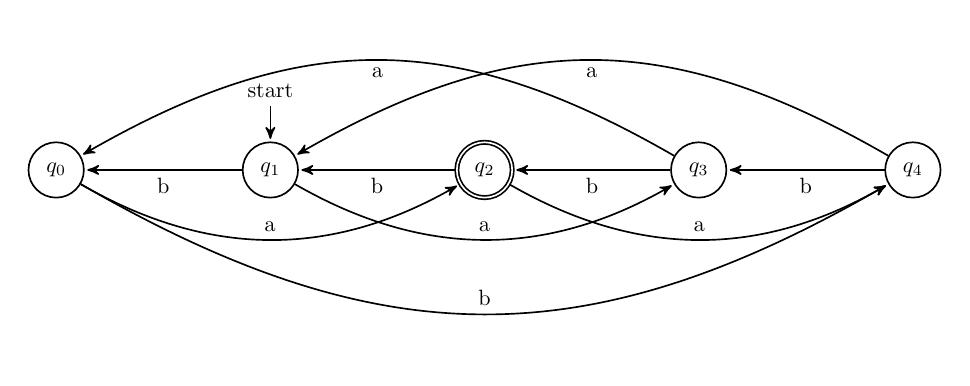
\begin{tikzpicture}[->,>=stealth',shorten >=1pt,auto,node distance=3.4cm,
                    semithick,every node/.style={scale=0.8}]
  \tikzstyle{every state}=[circle,text=black]

  \node[state] 				(A)             	{$q_0$};
  \node[initial above,state](B) [right of=A]	{$q_1$};
  \node[state,accepting]	(C) [right of=B]	{$q_2$};
  \node[state]        		(D) [right of=C]	{$q_3$};
  \node[state]        		(E) [right of=D]	{$q_4$};

  \path (A)	edge [bend right]				node {a} (C)
  			edge [bend right,looseness=1.1]	node {b} (E)
  		(B)	edge [bend right]				node {a} (D)
			edge							node {b} (A)
  		(C)	edge [bend right]				node {a} (E)
  			edge 							node {b} (B)
  		(D)	edge [bend right,looseness=1.1]	node {a} (A)
  			edge 							node {b} (C)
  		(E)	edge [bend right,looseness=1.1]	node {a} (B)
  			edge 							node {b} (D)
  ;
\end{tikzpicture}
\caption{Aufgabe 7a}
\end{figure}

\begin{figure}[!h]
\centering
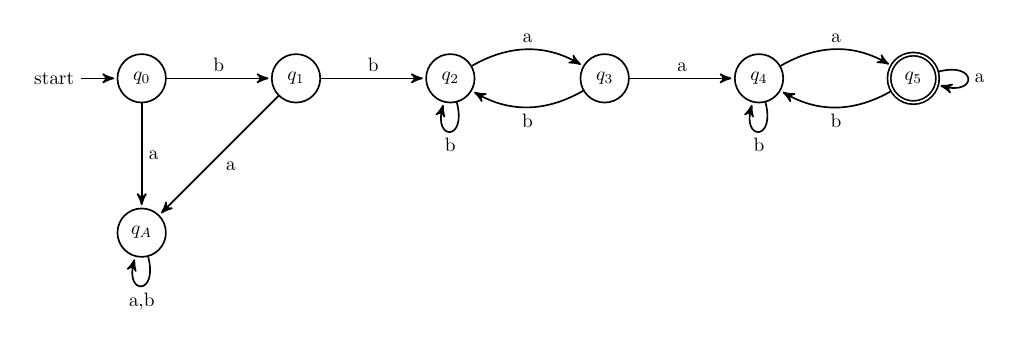
\begin{tikzpicture}[->,>=stealth',shorten >=1pt,auto,node distance=2.8cm,
                    semithick,every node/.style={scale=0.7}]
  \tikzstyle{every state}=[circle,text=black]

  \node[initial,state] 			(A)             	{$q_0$};
  \node[state]					(B) [right of=A]	{$q_1$};
  \node[state]					(C) [right of=B]	{$q_2$};
  \node[state]        			(D) [right of=C]	{$q_3$};
  \node[state]        			(E) [right of=D]	{$q_4$};
  \node[state,accepting]		(F) [right of=E]	{$q_5$};
  \node[state]        			(G) [below of=A]	{$q_A$};

  \path (A)	edge				node {a}	(G)
  			edge 				node {b}	(B)
  		(B)	edge 				node {a}	(G)
			edge 				node {b}	(C)
  		(C)	edge [bend left]	node {a}	(D)
  			edge [loop below]	node {b}	(C)
  		(D)	edge				node {a}	(E)
  			edge [bend left]	node {b}	(C)
  		(E)	edge [bend left]	node {a}	(F)
  			edge [loop below]	node {b}	(E)
 		(F)	edge [loop right]	node {a}	(F)
	  		edge [bend left]	node {b}	(E)
  		(G)	edge [loop below]	node {a,b}	(G)
  ;
\end{tikzpicture}
\caption{Aufgabe 7b}
\end{figure}

\end{homeworkProblem}

\begin{homeworkProblem}


\begin{figure}[!h]
\centering
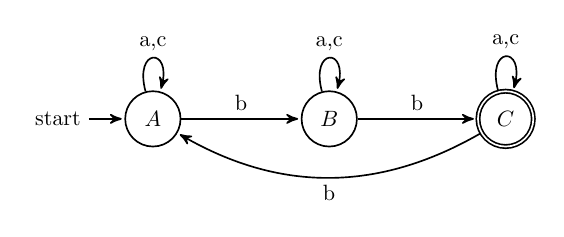
\begin{tikzpicture}[->,>=stealth',shorten >=1pt,auto,node distance=2.8cm,
                    semithick,every node/.style={scale=0.8}]
  \tikzstyle{every state}=[circle,text=black]

	\node[initial,state] 			(A)             	{$A$};
	\node[state]					(B) [right of=A]	{$B$};
	\node[state,accepting]			(C) [right of=B]	{$C$};

	\path	(A)		edge [loop above]		node {a,c}	(A)
	 				edge 					node {b}	(B)
	 		(B)		edge [loop above]		node {a,c}	(B)
	 				edge 					node {b}	(C)
			(C)		edge [loop above]		node {a,c}	(C)
	 				edge [bend left]		node {b}	(A)
  ;
\end{tikzpicture}
\caption{Aufgabe 8a, erster Teilgraph}
\end{figure}

\begin{figure}[!h]
\centering
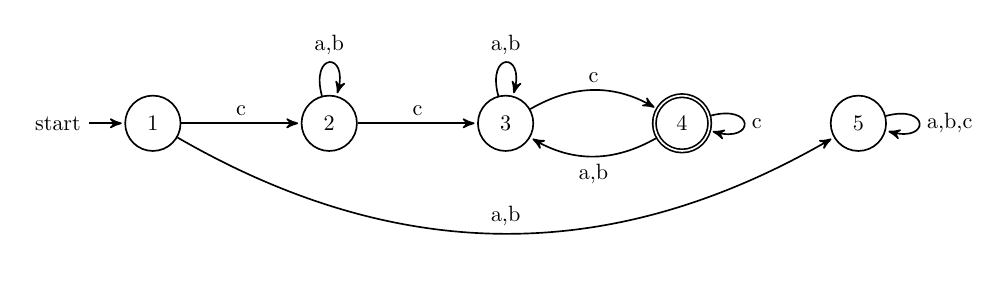
\begin{tikzpicture}[->,>=stealth',shorten >=1pt,auto,node distance=2.8cm,
                    semithick,every node/.style={scale=0.8}]
  \tikzstyle{every state}=[circle,text=black]

	\node[initial,state] 			(1)             	{$1$};
	\node[state]					(2) [right of=1]	{$2$};
	\node[state]					(3) [right of=2]	{$3$};
	\node[state,accepting]			(4) [right of=3]	{$4$};
	\node[state]					(5) [right of=4]	{$5$};

	\path	(1)		edge [bend right]		node {a,b}	(5)
	 				edge 					node {c}	(2)
	 		(2)		edge [loop above]		node {a,b}	(2)
	 				edge 					node {c}	(3)
			(3)		edge [loop above]		node {a,b}	(3)
	 				edge [bend left]		node {c}	(4)
			(4)		edge [loop right]		node {c}	(4)
	 				edge [bend left]		node {a,b}	(3)
			(5)		edge [loop right]		node {a,b,c}(5)
  ;
\end{tikzpicture}
\caption{Aufgabe 8a, zweiter Teilgraph}
\end{figure}

\begin{figure}[!h]
\centering
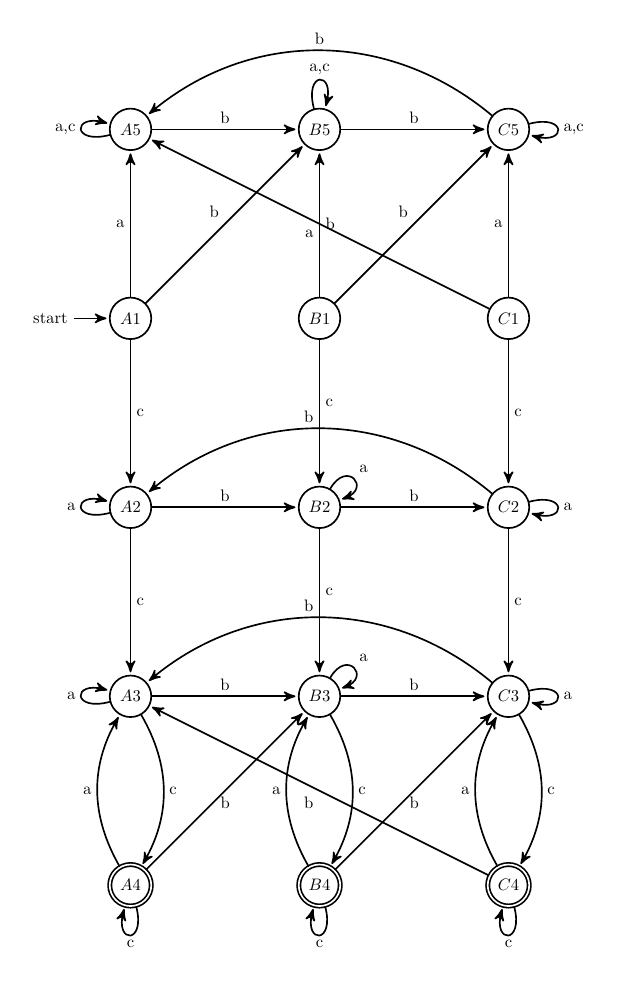
\begin{tikzpicture}[->,>=stealth',shorten >=1pt,auto,node distance=4cm,
                    semithick,every node/.style={scale=0.6}]
  \tikzstyle{every state}=[circle,text=black]

	\node[initial,state] 			(A1)             	{$A1$};
	\node[state]					(A2) [below of=A1]	{$A2$};
	\node[state]					(A3) [below of=A2]	{$A3$};
	\node[state,accepting]       	(A4) [below of=A3]	{$A4$};
	\node[state]        			(A5) [above of=A1]	{$A5$};
	\node[state] 					(B1) [right of=A1] 	{$B1$};
	\node[state]					(B2) [below of=B1]	{$B2$};
	\node[state]					(B3) [below of=B2]	{$B3$};
	\node[state,accepting]       	(B4) [below of=B3]	{$B4$};
	\node[state]        			(B5) [above of=B1]	{$B5$};
	\node[state] 					(C1) [right of=B1] 	{$C1$};
	\node[state]					(C2) [below of=C1]	{$C2$};
	\node[state]					(C3) [below of=C2]	{$C3$};
	\node[state,accepting]       	(C4) [below of=C3]	{$C4$};
	\node[state]        			(C5) [above of=C1]	{$C5$};
	
	\path	(A1)	edge 									node {a}	(A5)
			(A1)	edge 									node {b}	(B5)
			(A1)	edge 									node {c}	(A2)
			(A2)	edge [loop left]						node {a}	(A2)
			(A2)	edge									node {b}	(B2)
			(A2)	edge 									node {c}	(A3)
			(A3)	edge [loop left]						node {a}	(A3)
			(A3)	edge									node {b}	(B3)
			(A3)	edge [bend left]						node {c}	(A4)
			(A4)	edge [bend left]						node {a}	(A3)
			(A4)	edge [below]							node {b}	(B3)
			(A4)	edge [loop below]						node {c}	(A4)
			(A5)	edge [loop left]						node {a,c}	(A5)
			(A5)	edge 									node {b}	(B5)
			(B1)	edge [below left]						node {a}	(B5)
			(B1)	edge 									node {b}	(C5)
			(B1)	edge [above right]						node {c}	(B2)
			(B2)	edge [loop,out=60,in=20,looseness=6]	node {a}	(B2)
			(B2)	edge									node {b}	(C2)
			(B2)	edge [above right]						node {c}	(B3)
			(B3)	edge [loop,out=60,in=20,looseness=6]	node {a}	(B3)
			(B3)	edge									node {b}	(C3)
			(B3)	edge [bend left]						node {c}	(B4)
			(B4)	edge [bend left]						node {a}	(B3)
			(B4)	edge [below]							node {b}	(C3)
			(B4)	edge [loop below]						node {c}	(B4)
			(B5)	edge [loop above]						node {a,c}	(B5)
			(B5)	edge 									node {b}	(C5)
			(C1)	edge 									node {a}	(C5)
			(C1)	edge [right]							node {b}	(A5)
			(C1)	edge 									node {c}	(C2)
			(C2)	edge [loop right]						node {a}	(C2)
			(C2)	edge [bend right=40,above left]			node {b}	(A2)
			(C2)	edge 									node {c}	(C3)
			(C3)	edge [loop right]						node {a}	(C3)
			(C3)	edge [bend right=40,above left]			node {b}	(A3)
			(C3)	edge [bend left]						node {c}	(C4)
			(C4)	edge [bend left]						node {a}	(C3)
			(C4)	edge 									node {b}	(A3)
			(C4)	edge [loop below]						node {c}	(C4)
			(C5)	edge [loop right]						node {a,c}	(C5)
			(C5)	edge [bend right=40,above]				node {b}	(A5)
  ;
\end{tikzpicture}
\caption{Produktautomat}
\end{figure}

\end{homeworkProblem}

\begin{homeworkProblem}

$L_1=\{0^m1^n0^{m+n}\,|\,m, n \in \mathbb{N}\}$\\
Annahme: Sei $L_1$ regulär. Dann gibt es einen endlichen Automaten $A=(Q,\,\Sigma,\,\delta_A,\,q_0,\,F)$, sodass $L(A)=L$. Dieser hat $|Q_0|$ Zustände. Nach dem \textit{Pumping-Lemma} lässt sich ein $w$ mit $|w|=n_0$ in $w=xyz$ zerlegen und
\begin{enumerate}[(i)]
\item $|yx| \leq n_0$
\item $|x| \geq 1$
\item $\{yx^kz\,|\,k\in\mathbb{N}\} \subseteq L \quad\text{oder}\quad \{yx^kz\,|\,k\in\mathbb{N}\} \cup L = \emptyset$
\end{enumerate}
Jedes Wort $w$ der Länge $|w| \geq n_0$ muss also eine Zerlegung besitzen, die (i), (ii), (iii) erfülllt.\\
Sei $W=1^{n_0}0^{n_0}$, also $|w|=2*n \geq n_0$
\begin{align*}
\text{(i)}&\Rightarrow y=1^l,\;x=1^m\quad \text{mit }l,\,m \in \mathbb{N}\\
\text{(iii)}&\Rightarrow \text{Da } w=1^{n_0}0^{n_0}\in L, \text{ ist } \{yx^kz\,|\,k\in\mathbb{N}\}=\{1^l\left(1^m\right)^k0^{n_0}\} \subseteq L 
\end{align*}
Aber: für $k=0$ ist $w=yz=1^{n_0-m}0^{n_0} \not\in L$\\
Wir haben einen Widerspruch, daher war die Annahme, dass L regulär ist, falsch.
\end{homeworkProblem}

\end{document}
